\ifdefined\included
\else
\documentclass[french, a4paper, 11pt, twoside, pdftex]{StyleThese}
\usepackage{iflang}
\usepackage{bibentry}



%\usepackage[sectionbib]{chapterbib}          % Cross-reference package (Natural BiB)
%\usepackage{natbib}                  % Put References at the end of each chapter
%\usepackage{bibunits}
% Do not put 'sectionbib' option here.
% Sectionbib option in 'natbib' will do.


\usepackage{fancyhdr}                    % Fancy Header and Footer

\usepackage[utf8]{inputenc}
\usepackage[T1]{fontenc}
\usepackage[french]{babel} %
\usepackage{lmodern} \normalfont %to load T1lmr.fd 
\DeclareFontShape{T1}{cmr}{b}{sc} { <-> ssub * cmr/bx/sc }{}
%\hyphenation{gar}

\usepackage{amsmath,amssymb}             % AMS Math
\usepackage{nicefrac}
\usepackage{siunitx}					%% Unites Math SI

\usepackage{blindtext}

\usepackage{datetime}

\usepackage{lipsum} 

\usepackage[inline]{enumitem}

\usepackage{hhline}
%\usepackage[left=1.5in,right=1.3in,top=1.1in,bottom=1.1in]{geometry}
\usepackage[left=1.5in,right=1.3in,top=1.1in,bottom=1.1in,includefoot,includehead,headheight=13.6pt]{geometry}

%%\renewcommand{\baselinestretch}{1.05}

%%%%%%%% Multi-figures avec sub-captions
\usepackage{caption}
\usepackage{subcaption}

% Table of contents for each chapter

\usepackage[nottoc, notlof, notlot]{tocbibind}
\usepackage[nohints]{minitoc}
\setcounter{minitocdepth}{2}
\mtcindent=15pt
% Use \minitoc where to put a table of contents

\usepackage{aecompl}

%% Package cosmetic meilleur layout du texte en jouant sur le spacing par caractères
\usepackage[activate={true,nocompatibility},final,tracking=true,kerning=true,factor=1100,stretch=10,shrink=10]{microtype}
\usepackage[absolute,overlay]{textpos} 
\setlength{\TPHorizModule}{\paperwidth}\setlength{\TPVertModule}{\paperheight}
\sloppy

%%%%%%%%%%% JOLIS TABLEAUX
\usepackage{tabularx}		%\usepackage{tabular}
\usepackage{longtable}
\usepackage{multirow}
\newcommand{\mc}{\multicolumn} 
\newcommand{\mr}[2]{\multirow{#1}{*}{#2}} 	\newcommand{\mrQ}{\multirow{-4}{*}}
\usepackage{booktabs}

\usepackage[usenames,dvipsnames]{xcolor} 

\makeatletter
\newcommand{\ccolor}[3][]{%
	\kern-\fboxsep
	\if\relax\detokenize{#1}\relax
	\expandafter\@firstoftwo
	\else
	\expandafter\@secondoftwo
	\fi
	{\colorbox{#2}}%
	{\colorbox[#1]{#2}}%
	{#3}\kern-\fboxsep
}
\makeatother

%%%%% Insertion graphiques format PGF
\usepackage{pgfplots}
\pgfplotsset{width=\linewidth, compat=1.16}%, compat=1.17}
\usepackage{adjustbox}          %%% PERMET DE LES RECADRER + FACILEMENT


%%%%%%%%%% Bullets de listes sans saut de ligne %%%%%%%%%%
\usepackage{xparse}

\ExplSyntaxOn%
\seq_new:N \l_local_enum_seq

\newcommand{\storethestuff}[1]{%
  \seq_set_from_clist:Nn \l_local_enum_seq {#1}%
}

\newcommand{\dotheenumstuff}{%
\int_zero:N \l_tmpa_int
\seq_map_inline:Nn \l_local_enum_seq {%
    \int_incr:N \l_tmpa_int% Increase the counter
    \item ##1
    % Check whether the list has reached the end -- if so, use '.' instead of ','
    %\int_compare:nNnTF 
    % { \l_tmpa_int } < {\seq_count:N \l_local_enum_seq} 
    % {,} {.}
  }
}
\ExplSyntaxOff

\NewDocumentCommand{\linebullets}{+m}{%
  \storethestuff{#1}%
  \begin{enumerate*}[label={\alph*)},font={\bfseries},itemjoin={{, }}]
    \dotheenumstuff%
  \end{enumerate*}
}

\newcommand{\cmnt}[1]{}  %%%%% AJOUT DE COMMENTAIRE MULTILIGNES


%%%%%%%%%% ECRITURE CARACTERES DANS UN CERCLE %%%%%%%%%%
%\def\circleTxt[#1]{\raisebox{.5pt}{\textcircled{\raisebox{-1pt}{#1}}}}
\newcommand{\ctxt}[1]{\raisebox{.5pt}{\textcircled{\raisebox{-1.2pt}{#1}}}}
% Glossary / list of abbreviations

\usepackage[intoc]{nomencl}
\IfLanguageName{english}{%
\renewcommand{\nomname}{Glossary}
}{ %
\renewcommand{\nomname}{Liste des Abréviations}
}

\makenomenclature

% My pdf code

\usepackage{ifpdf}

\ifpdf
  \usepackage[pdftex]{graphicx}
  \DeclareGraphicsExtensions{.pdf,PDF,.png,PNG,.jpg,JPG}
  \usepackage[pagebackref,hyperindex=true]{hyperref} %% use \autoref{} instead of Table~\ref{}.
  \usepackage{tikz}
  \usetikzlibrary{arrows,shapes,calc}
\else
  \usepackage{graphicx}
  \DeclareGraphicsExtensions{.ps,.eps}
  \usepackage[a4paper,dvipdfm,pagebackref,hyperindex=true]{hyperref}
\fi

\graphicspath{{.}{schemas/}{graphiques/}{tables/}}

%% nicer backref links. NOTE: The flag ThesisInEnglish is used to define the
% language in the back references. Read more about it in These.tex

\IfLanguageName{english}{
\renewcommand*{\backref}[1]{}
\renewcommand*{\backrefalt}[4]{%
\ifcase #1 %
(Not cited.)%
\or
(Cited in page~#2.)%
\else
(Cited in pages~#2.)%
\fi}
\renewcommand*{\backrefsep}{, }
\renewcommand*{\backreftwosep}{ and~}
\renewcommand*{\backreflastsep}{ and~}
}{
\renewcommand*{\backref}[1]{}
\renewcommand*{\backrefalt}[4]{%
\ifcase #1 %
(Non cité.)%
\or
(Cité en page~#2.)%
\else
(Cité en pages~#2.)%
\fi}
\renewcommand*{\backrefsep}{, }
\renewcommand*{\backreftwosep}{ et~}
\renewcommand*{\backreflastsep}{ et~}
}

% Links in pdf
\usepackage{color}
\definecolor{linkcol}{rgb}{0,0,0.4} 
\definecolor{citecol}{rgb}{0.5,0,0} 
\definecolor{linkcol}{rgb}{0,0,0} 
\definecolor{citecol}{rgb}{0,0,0}
% Change this to change the informations included in the pdf file

\hypersetup
{
bookmarksopen=true,
pdftitle="Prévention des fautes temporelles sur architectures multicœur pour les systèmes à criticité mixte",
pdfauthor="Daniel LOCHE", %auteur du document
pdfsubject="Thèse", %sujet du document
%pdftoolbar=false, %barre d'outils non visible
pdfmenubar=true, %barre de menu visible
pdfhighlight=/O, %effet d'un clic sur un lien hypertexte
colorlinks=true, %couleurs sur les liens hypertextes
pdfpagemode=UseNone, %aucun mode de page
%pdfpagelayout=DoublePage, %ouverture en simple page
pdffitwindow=true, %pages ouvertes entierement dans toute la fenetre
linkcolor=linkcol, %couleur des liens hypertextes internes
citecolor=citecol, %couleur des liens pour les citations
urlcolor=linkcol %couleur des liens pour les url
}

% definitions.
% -------------------

\setcounter{secnumdepth}{3}
\setcounter{tocdepth}{2}

% Some useful commands and shortcut for maths:  partial derivative and stuff

\newcommand{\pd}[2]{\frac{\partial #1}{\partial #2}}
\def\abs{\operatorname{abs}}
\def\argmax{\operatornamewithlimits{arg\,max}}
\def\argmin{\operatornamewithlimits{arg\,min}}
\def\diag{\operatorname{Diag}}
\newcommand{\eqRef}[1]{(\ref{#1})}
\newcommand{\nline}{\smallbreak\noindent}

\usepackage{rotating}                    % Sideways of figures & tables

% \usepackage{txfonts}                     % Public Times New Roman text & math font
  
%%% Fancy Header %%%%%%%%%%%%%%%%%%%%%%%%%%%%%%%%%%%%%%%%%%%%%%%%%%%%%%%%%%%%%%%%%%
% Fancy Header Style Options

\pagestyle{fancy}                       % Sets fancy header and footer
\fancyfoot{}                            % Delete current footer settings

%\renewcommand{\chaptermark}[1]{         % Lower Case Chapter marker style
%  \markboth{\chaptername\ \thechapter.\ #1}}{}} %

%\renewcommand{\sectionmark}[1]{         % Lower case Section marker style
%  \markright{\thesection.\ #1}}         %

\fancyhead[LE,RO]{\bfseries\thepage}    % Page number (boldface) in left on even
% pages and right on odd pages
\fancyhead[RE]{\bfseries\nouppercase{\leftmark}}      % Chapter in the right on even pages
\fancyhead[LO]{\bfseries\nouppercase{\rightmark}}     % Section in the left on odd pages

\let\headruleORIG\headrule
\renewcommand{\headrule}{\color{black} \headruleORIG}
\renewcommand{\headrulewidth}{1.0pt}
\usepackage{colortbl}
\arrayrulecolor{black}

\fancypagestyle{plain}{
  \fancyhead{}
  \fancyfoot{}
  \renewcommand{\headrulewidth}{0pt} %%%%%%%%%%%%%%%%%%%%%%%%%%%%%%%%%%%%%%%%%%%%%%%%%%%%%%%%%%%%%%%%%%%%%%%%%%%%%%%%%%%%%
}

%\usepackage{MyAlgorithm}
%\usepackage[noend]{MyAlgorithmic}
%\usepackage[ED=EDSYS-SystEmb, Ets=INP]{tlsflyleaf}

%%% Clear Header %%%%%%%%%%%%%%%%%%%%%%%%%%%%%%%%%%%%%%%%%%%%%%%%%%%%%%%%%%%%%%%%%%
% Clear Header Style on the Last Empty Odd pages
\makeatletter

\def\cleardoublepage{\clearpage\if@twoside \ifodd\c@page\else%
  \hbox{}%
  \thispagestyle{empty}%              % Empty header styles
  \newpage%
  \if@twocolumn\hbox{}\newpage\fi\fi\fi}

\makeatother
 
%%%%%%%%%%%%%%%%%%%%%%%%%%%%%%%%%%%%%%%%%%%%%%%%%%%%%%%%%%%%%%%%%%%%%%%%%%%%%%% 
% Prints your review date and 'Draft Version' (From Josullvn, CS, CMU)
\newcommand{\reviewtimetoday}[2]{\special{!userdict begin
    /bop-hook{gsave 20 710 translate 45 rotate 0.8 setgray
      /Times-Roman findfont 12 scalefont setfont 0 0   moveto (#1) show
      0 -12 moveto (#2) show grestore}def end}}
% You can turn on or off this option.
% \reviewtimetoday{\today}{Draft Version}
%%%%%%%%%%%%%%%%%%%%%%%%%%%%%%%%%%%%%%%%%%%%%%%%%%%%%%%%%%%%%%%%%%%%%%%%%%%%%%% 

\newenvironment{maxime}[1]
{
	\def\Arg{#1}
\vspace*{0cm}
\hfill
\begin{minipage}{0.6\textwidth}%
%\rule[0.5ex]{\textwidth}{0.1mm}\\%
\hrulefill $\:$ \\%$\:$ {\bf #1}\\
%\vspace*{-0.25cm}
\it 
}%
{%
	
\hrulefill $\:$ {\bf \Arg}
\vspace*{0.5cm}%
\end{minipage}
}

\let\minitocORIG\minitoc
\renewcommand{\minitoc}{\minitocORIG \vspace{1.5em}}

%\usepackage{slashbox}

\newenvironment{bulletList}%
{ \begin{list}%
	{$\bullet$}%
	{\setlength{\labelwidth}{25pt}%
	 \setlength{\leftmargin}{30pt}%
	 \setlength{\itemsep}{\parsep}}}%
{ \end{list} }


%%%%%%% Outils pour \comment \alert \add %%%%%
\usepackage{easyReview}
\usepackage{soulutf8} % for accented letters

\let\newalert\alert
\renewcommand{\alert}[1]{\textit{\newalert{#1}}}

%\usepackage[commandnameprefix=ifneeded]{changes} %% \chhighlight and \chcomment to avoid collision with easyReview
\renewcommand{\epsilon}{\varepsilon}

% centered page environment

\newenvironment{vcenterpage}
{\newpage\vspace*{\fill}\thispagestyle{empty}\renewcommand{\headrulewidth}{0pt}}
{\vspace*{\fill}}

\usepackage{tablefootnote}

%%%%%% MISE EN FORME CADRES DEFINITIONS/THEOREMES/LEMES %%%%%%%%%%
\usepackage{amsthm}  % for theoremstyle

\theoremstyle{plain} 
\newtheorem{theorem}{Théorème}[section]
\newtheorem{corollary}{Corolaire}[theorem]

%\theoremstyle{lemma}
%\newtheorem{lemma}[theorem]{Lemme}


\theoremstyle{definition}
\newtheorem{definition}[theorem]{Définition}


\cmnt{
	\usepackage{ntheorem} %\usepackage{amsthm}  % for theoremstyle
	%\usepackage{mdframed}
	\usepackage[most]{tcolorbox}
	
	\theoremstyle{plain} 
	\theoremindent20pt
	\theoremheaderfont{\normalfont\bfseries\hspace{-\theoremindent}}
	\newtheorem{theorem}{Théorème}[section]
	\newtheorem{corollary}{Corolaire}[theorem]
	
	\theoremstyle{plain}
	\newtheorem{lemma}[theorem]{Lemme}
	
	
	\tcolorboxenvironment{theorem}{
		blanker,
		breakable,
		before skip=\topsep,
		after skip=\topsep,
		borderline west={1pt}{10pt}{double, shorten <=12pt}
	}
	
	\theorembodyfont{\normalfont}
	\theoremindent20pt
	\theoremheaderfont{\normalfont\bfseries\hspace{-\theoremindent}}
	\newtheorem{definition}[theorem]{Définition}
	
	
	\tcolorboxenvironment{definition}{
		blanker,
		breakable,
		before skip=\topsep,
		after skip=\topsep,
		borderline west={1pt}{10pt}{shorten <=12pt}
	}
}

\cmnt{ 
	\begin{theorem}
		Ceci est un Théorème.
	\end{theorem} 
	
	\begin{corollary}
		Ceci est un Corollaire.
	\end{corollary}
	
	\begin{definition}
		Ceci est une Définition.
	\end{definition}
	
	\begin{lemma}
		Ceci est un Lemme.
	\end{lemma}
}

\def\UrlBigBreaks{\do\/\do-\do:}
\usepackage{url}

\sloppy
\begin{document}
\setcounter{chapter}{3} %% Numéro du chapitre précédent ;)
\dominitoc
\faketableofcontents
\fi

\chapter{Protocole et démarche expérimentale} \label{chap:4_ProtocolExpe}
\minitoc

Jusqu'à présent, nous avons fait un état des lieux des enjeux liés à l'usage des calculateurs multicœurs dans le cadre d'applications à criticité mixte et en dégager une problématique. Après une revue des solutions existantes dans le domaine, nous avons présenté dans le \hyperref[chap:3_PrincipeArchi]{Chapitre précédent} nos hypothèses de travail ainsi que le modèle de notre mécanisme d'évitement de fautes temporelles basé sur la surveillance d'une Chaîne de tâches critiques. Nous allons maintenant aborder une méthodologie de mise en service et de calibration du mécanisme pour un cas d'application. Cela nous permettra d'identifier les fondamentaux qui serviront au cas d'étude du \hyperref[chap:5_ImplementationCase]{Chapitre suivant}.

Notre proposition méthodologique repose sur 3 grandes phases de conception. Nous développerons successivement les exigences liées à la phase de Conception et de caractérisation d'un cas de test. L'objectif de cette démarche expérimentale est de caractériser un jeu de tâches au regard de sa propension à provoquer des interférences, et sa sensibilités aux-dites interférences. 

Les étapes de calibration et d'ajustement du mécanisme ont pour but d'implémenter et de configurer le mécanisme de Surveillance et de Contrôle pour l'implémenter sur un système à criticité duale donné.

Enfin la phase de vérification consiste à mesurer les propriétés de notre mécanisme ainsi configuré, pour un système donné. Il s'agit de mesurer et d'analyser plusieurs métriques : la Qualité, la Fiabilité et la Performance, au regard de la capacité à respecter l'échéance bout-en-bout de la chaîne de tâche, à limiter le temps d'arrêt des tâches non critiques, et à éviter les faux-positifs.



\pagebreak

\section{Principe Général et Objectifs}
        L'objectif de ce Chapitre est de présenter notre protocole expérimental, pour répondre à deux objectifs~: 
        \begin{itemize}
        	\item Le premier de caractériser un système de tâches donné pour y définir une chaîne de tâches critiques ainsi que le profil temporel des différentes tâches. 
        	\item         Le second de calibration et de test de l'Agent de Surveillance et Contrôle.
        \end{itemize}
        Il est important de préciser que notre méthode se décompose en ces deux intérêts bien distincts. En effet, une première partie du protocole général qui a été mis en place dans le cadre de ces travaux s'inscrit dans la phase de conception et de spécification. Cette partie se destine à la mise en place d'un banc expérimental qui ne repose pas sur un système déjà existant. De fait, en l'absence d'un système réel avec ses  spécifications propres sur lesquelles se baser, il nous faut recréer un cas de test et donc en fixer les contraintes temporelles qui soient cohérentes avec les caractéristiques d'exécution du logiciel qui est utilisé. En conséquence, l'ajout d'étapes méthodologiques a été nécessaire pour donner des spécifications cohérentes à ce cas d'utilisation et connaître le comportement temporel de notre cas de test. 
        Une fois cet aspect traité, la seconde partie du protocole expérimental présente normalement les étapes nécessaires qui doivent s'intégrer au processus de développement et d'intégration préexistant pour y ajouter l'Agent de Surveillance et Contrôle, le calibrer et le tester.
        
        Ce chapitre se divise donc en deux sections qui correspondent aux processus susmentionnés. Ils permettront de définir en amont du développement et de l'intégration de la solution quelles sont les données dont nous disposons en entrée et quels sont les résultats attendus en sortie de chaque étape du processus. Dans un dernier temps, nous agrégerons tout cela pour constituer un protocole expérimental global qui sera celui-utilisé pour la suite dans le cadre de notre mise en application.
        
        \section{Protocole de conception d'un cas de test}
        
        Le protocole de conception d'un cas de test proposé se divise en 5 phases distinctes. L'objectif est d'extraite à partir d'un set de tâches logicielles donné un ensemble de tâches dont on connaît les profils d'exécution et la sensibilité aux interférences dans un cas artificiellement stressé au maximum. Ces informations permettent dans un second temps de sélectionner de façon pertinente les tâches qui constitueront un cas de test sur lequel implémenter le mécanisme de Surveillance et Contrôle. Le cas de test doit se composer d'une part d'un ensemble de tâches critiques d'une part et non critiques d'autre part. La caractérisation sert à identifier les tâches suivant des critères de stabilité et fiabilité (c.-à-d. variabilité d'exécution pour une même entrée), sensibilité aux interférences et part d'interférences générées par l'usage de ressources partagées.
        
        Ce processus est relativement important pour quantifier les effets de notre mécanisme. De fait, la problématique d'interférences inter-tâches à laquelle nous essayons de répondre est hautement dépendante du comportement des tâches, notamment par leur usage des ressources partagées. Pour cette raison, il est important d'avoir une bonne connaissance sur le logiciel sur lequel s'intègre un mécanisme censé limiter les conséquences de ces interférences. Cette démarche de caractérisation d'un jeu de tâches peut avoir son importance de la même manière pour un cas d'application industrielle déjà existant. De fait, particulièrement dans l'usage de logiciel en boite noire, il est essentiel d'avoir une bonne maîtrise de ses caractéristiques d'exécution. Particulièrement dans la connaissance du taux d'utilisation de chaque ressource et de leur influence sur les temps d'exécution. Cela offre des éléments de décision pour l'allocation physique et d'ordonnancement des tâches. De cette façon le risque d'erreur d'estimation ou d'effets de bords dans les choix d'intégration peuvent être anticipé, voire limité.
        
        Dans le cadre de nos expérimentations, l'objectif de ce protocole est de mesurer les métriques propres aux interférences inter-tâches~: l'empreinte mémoire des tâches, le nombre de lectures/écritures, le nombre d'appels système, la puissance de calcul utilisée (taux CPU) et bien entendu les temps d'exécution et la sensibilité à l'application d'un stress sur les ressources partagées. De cette analyse, on se focalisera donc sur l'exploitation des tâches qui sont relativement sensibles à ces interférences d'une part, et à celles qui ont une forte empreinte mémoire et/ou une grande demande en ressources de calcul d'autre part. Cette démarche permet aussi pour un jeu de tâches préexistant, qui n'a pas été conçu pour un contexte de tâches temps-réel tel qu'on l'envisage, d'éliminer celles qui ont un comportement non maîtrisé qui ne correspond pas à un minimum que l'on serait en droit d'espérer de logiciel embarqué (par exemple une tâche qui aurait des variations de temps d'exécution sans interférences d'un ou plusieurs ordres de grandeur entre les millisecondes et la seconde).
        
        \begin{table}[ht]
        	\centering
        	\caption{Protocole de caractérisation d'un jeu de tâches}
        	\label{tab:tableprotocoledesign}
        	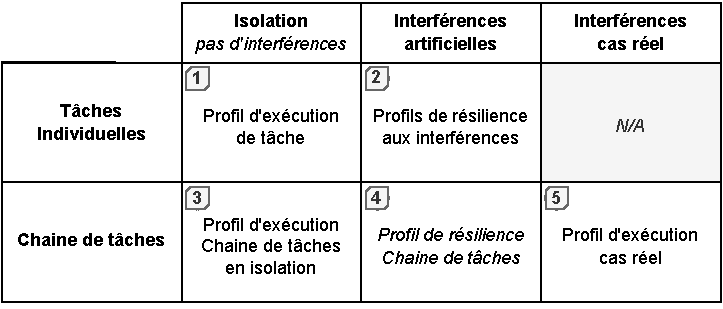
\includegraphics[width=0.8\linewidth]{tables/Table_Protocole_Design}
        \end{table}
             
        Pour arriver à cet objectif, nous allons travailler sur deux paramètres dans le cadre de ce protocole expérimental. D'une part nous allons faire varier la charge utile, qui est le logiciel monitoré pour en tirer ses caractéristiques, et d'autre part nous modifions les interférences -- le stress -- subi par la charge utile. Les différentes étapes du protocole sont agrégées dans le Tableau~\ref{tab:tableprotocoledesign}. La charge utile sera au choix soit une tâche spécifique, soit une chaîne de tâches telle que définie dans le chapitre précédent, tandis qu'elle sera soumise soit à~: \begin{enumerate}[label=\bfseries\alph*)] 
        	\item aucune interférence, donc en isolation,
        	\item des interférences imposées de façon artificielles par le biais de logiciels dédiés (comme \texttt{stress-ng} sous Linux) pour stresser au maximum le système,
        	\item les autres tâches du système, qui impliquent leurs propres interférences sur les ressources partagées.
        \end{enumerate}
    
        Suivant ces paramètres, le protocole de caractérisation se compose de cinq étapes, d'abord en caractérisant les tâches de façon individuelles, ensuite en caractérisant la chaîne de tâches critiques et enfin en vérifiant la pertinence des choix des tâches critiques et non critiques et de leurs paramètres, au regard de l'ordonnançabilité et de la présence d'interférences logicielles~: 
        \begin{itemize}
        	\item Profil d'exécution de chaque tâche
	        \begin{enumerate}[label=\large\ctxt{\arabic*}]
	        	\item tâches individuelles exécutées en isolation
	        	\item tâches individuelles exécutées avec stress imposé
	        \end{enumerate}
        	\item Profil d'exécution de la chaîne de tâches critiques
        	\begin{enumerate}[resume*]
        		\item chaîne de tâches en condition d'exécution en isolation
        		\item chaîne de tâches exécutée avec le stress artificiel
        	\end{enumerate}
        	\item Set de tâche complet
        	\begin{enumerate}[resume*]
        		\item chaîne de tâches \& tâches non-critiques qui constituent le cas de test 
        	\end{enumerate}
        \end{itemize}
    

	\subsection{Profil des tâches}
		Cette phase est nécessaire de façon à déterminer le profil d'exécution des tâches qui sont à notre disposition pour former un cas de test. Bien entendu, dans l'éventualité où l'on disposerait d'ores et déjà d'un jeu de tâches accompagné de leurs spécifications, il n'est pas nécessaire de réaliser ces étapes de profilage des tâches dans l'objectif d'y réaliser une sélection de tâches critiques et non-critiques pour constituer notre cas de test. Il est possible de passer directement à l'étape~\ctxt{3} pour caractériser la chaîne de tâches critiques au regard du système et vérifier la pertinence d'implémenter un mécanisme de surveillance et contrôle selon les variations de temps de réponse sur les tâches critiques. 
		
		Ceci étant dit, ces étapes peuvent tout de même être intéressantes dans un cas industriel où le jeu de tâches est déjà déterminé et spécifié en avance. Comme mentionné plus haut, cela peut apporter une connaissance plus détaillée des tâches et donc aider dans l'anticipation de risques d'interférences et dans le choix de l'allocation des tâches pour le prévenir.
		
		L'objectif de la phase de profilage est donc d'avoir les connaissances suffisantes sur les tâches en termes de temps d'exécution à la fois en cas optimal (aucune interférence) et au cas où la tâche subit un stress sur l'utilisation de ressources partagées. À cet effet, on peut mesurer des éléments subsidiaires tels que l'espace mémoire occupé, le nombre d'appels systèmes et le profil de lecture/calcul/écriture des tâches pour une analyse plus fine. À l'issue de ces tests, on doit être capable de spécifier quelles seront les tâches sélectionnées pour constituer le cas de test. Certaines tâches seront simplement éliminées à cause de caractéristiques compromettantes telles que des temps d'exécution trop variables ou différents des autres tâches pour cohabiter ou des problèmes de non-déterminisme. D'autres pourront être éligibles en tant que tâches critiques, de par une bonne fiabilité d'exécution. Enfin et surtout, il faudra inclure dans les tâches non-critiques au moins une part de tâches qui ont une forte influence sur l'utilisation des ressources partagées. Elles seront donc propices au déclenchement d'interférences sur les tâches critiques. Cette phase inclut donc les étapes \ctxt{1} et \ctxt{2}.
		
		\paragraph{\ctxt{1} - Tâches en Isolation}
			
			Cette première phase du processus consiste à exécuter une tâche individuelle sur la plateforme d'intégration en lui fournissant des données d'entrée de façon périodique. Sont mesurées les informations susmentionnées pour un nombre représentatif d'exécutions au regard de la variété possible des données d'entrée. 
			
			Dans le cas où l'on ne connaît pas l'ordre de grandeur des temps d'exécutions, il faudra prendre dans un premier temps une période d'exécution arbitraire relativement large (toutes les secondes par exemple). Il est possible ensuite de réduire ce temps pour que les tests soient plus rapides (toutes les 50ms pour une tâche qui prend autour de 20ms typiquement). Si le jeu de tâches dispose d'ores-et-déjà de spécifications sur les temps d'exécutions moyens, il est possible de choisir directement une valeur proche avec une marge de sûreté pour être sûr de la complétion systématique de la tâche.
			
			Ces mesures expérimentales doivent être reproduites pour chaque tâche, de façon à obtenir une table des caractéristiques de chaque tâche en isolation.
                    
    	\paragraph{\ctxt{2} - Tâches avec stress imposé artificiel}
    		
    		De la même façon que pour l'étape précédente, l'objectif est d'obtenir les mêmes informations de profilage des tâches dans une mise en situation où le matériel est soumis à un niveau de stress élevé sur l'utilisation des caches, des entrées/sorties et en usage CPU, tandis que la tâche testée est exécutée périodiquement pour une durée suffisante de façon à obtenir un échantillon représentatif. Cela est dépendant du système et de la tâche en question.
    		
    		Les étapes avec un stress imposé de façon artificielle sur le matériel par l'usage d'outils dédiés au stress. Plusieurs solutions sont possibles selon la plateforme de développement impliquée (matériel et logiciel). Pour mentionner quelques exemples, dans le cadre des travaux de~\cite{blin_maximizing_2016} des tâches dédiées ont été codées en assembleur pour effectuer des cycles d'accès mémoire sur une plateforme multicœur SABRE Lite. Sur des systèmes basés sur UNIX, il existe des outils comme \texttt{stress-ng}~\cite{king_stress-ng_2019} qui offrent toute une librairie d'utilitaires pour stresser des éléments spécifiques du processeur. Des travaux comme ceux de \cite{girbal_metrics_2018} proposent aussi un environnement de mesure des métriques d'exécution pour l'analyse de systèmes temps-réel sur multicœur.  
%%%% Je n'ai pas trouvé ECRTS 2021 (2020 ?) de Daniel Garcia Perez suggéré par ici...
	    	À l'issue de ces deux étapes de caractérisation, on dispose d'une matrice des caractéristiques du jeu de tâches qui inclut pour chaque tâche ses caractéristiques de temps de réponse en isolation et avec interférences sur les ressources partagées (i.e. stressée) et les compteurs pertinents (appels systèmes, préemptions...), tel qu'illustré dans le~\autoref{tab:tasksCaracs}. On y trouve les temps d'exécution minimum, médian, moyen et maximum, le nombre d'appels système, et éventuellement d'autres métriques propres à l'environnement d'exécution si elles sont pertinentes (nombre d'appels à un composant spécifique du firmware par exemple). 
	    	    	
	    	À partir de ces données, on peut alors identifier~:
	    	\begin{enumerate}
	    		\item Les tâches qui ne sont pas adaptées à nos besoins pour un cas de test. Soit parce que leurs temps d'exécution ne sont pas à la bonne échelle, c'est-à-dire avec des écarts d'ordre de grandeur trop importants. Par exemple des tâches trop macroscopiques qui prennent plusieurs secondes de calcul alors que le reste du système de tâche est composé de micro-tâches monofonctionnelles qui s'exécutent en quelques dizaines de millisecondes. Soit parce qu'elles ont été codées d'une manière qui ne semble pas acceptable, par exemple avec une surutilisation des appels système, qui provoquent des ralentissements indésirables trop dépendants du système d'exploitation.
	    		\item Les tâches qui sont appropriées pour servir de tâches non critiques qui vont provoquer des interférences. Ces dernières peuvent avoir des variations de temps d'exécution non négligeables et utiliser des ressources partagées.
	    		\item Enfin, les tâches qui peuvent servir en tant que tâches critiques, qui représentent alors a minima des tâches temps-réel souple avec peu, voire pas d'appels système et un fonctionnement maîtrisé en isolation (variations de temps d'exécution raisonnables), et potentiellement sensibles à des interférences, donc avec une variation non négligeable du temps d'exécution médian entre les 2 conditions de test.
	    	\end{enumerate}
	    		
	    	\begin{table}[h]
				\centering
				\caption{Template type des données de caractérisation des tâches}
				\label{tab:tasksCaracs}
				\begin{tabular}{@{}c cc ccc c ccc@{}}
					\toprule
					\mr{2}{Tâche}& \mr{2}{Appels Sys.} & \mr{2}{Autres appels} & \mc{3}{c}{en isolation} & \phantom{} & \mc{3}{c}{stressé} \\
					\cmidrule{4-6} \cmidrule{8-10}
					& & & $ t_{min} $ & $ t_{max} $ & $ t_{med} $ &\phantom{} &  $ t_{min} $ & $ t_{max} $ & $ t_{med} $  \\
					\midrule
					$\tau_1$ & -- & -- & -- & -- & -- &  & -- & -- & -- \\
					... 	 & -- & -- & -- & -- & -- &  & -- & -- & -- \\
					$\tau_n$ & -- & -- & -- & -- & -- &  & -- & -- & -- \\
					\bottomrule
				\end{tabular}
			\end{table} 
    		
    		À l'issue de cette sélection, on a donc à disposition un jeu de tâches, qui va être constitué d'une liste de \textbf{tâches non critiques} avec une période d'exécution pour chacune d'entre elle, et une liste de \textbf{tâches critiques} qui constituent la chaîne de tâches, qui doit donc inclure toutes les données relatives à la chaîne de tâches : période d'exécution de chaque tâche, mais aussi contraintes de précédence et échéance de temps de réponse bout-en-bout.
    		
    		Il s'avère que cette dernière donnée va être hautement dépendante des spécifications système dans le cadre d'un cas applicatif réel. 
    		
    		Dans une situation purement expérimentale où il nous faut constituer nous même le cas de test, cette donnée de temps de réponse bout-en-bout doit être fixée arbitrairement. Par conséquent, il va falloir là encore proposer une façon de fixer cette contrainte, ou au moins en définir un ordre de grandeur qui pourra être ajusté selon la difficulté que l'on souhaite imposer au test. Plus cette échéance est courte, plus il sera difficile de la garantir au regard des pires temps d'exécution des tâches et des risques d'allongement d'exécution inhérents notamment aux interférences
    		
                    
    \subsection{Profil du cas de test et Chaîne de tâches}
    
L'objectif de cette seconde phase de caractérisation consiste justement à caractériser plus globalement les tâches sélectionnées, notamment par la vérification de l'ordonnançabilité et de la contrainte de temps de réponse bout-en-bout de la chaîne. Il s'agit des étapes \ctxt{3}, \ctxt{4} et \ctxt{5} du protocole.

		\paragraph{\ctxt{3} - Chaîne de tâches critiques en isolation}
		Il est important de tester l'exécution de la chaîne de tâches en isolation, c'est-à-dire sans aucune interférence provenant des autres tâches qui doivent être intégrées. Cette étape permet de vérifier l'absence d'effets de bord entre la situation où les tâches étaient testées individuellement et le cas où la chaîne de tâches est exécutée sans aucune autre tâche non critique, donc en isolation. Le mode que l'on souhaite caractériser ici correspond, dans le cadre de l'utilisation du mécanisme de surveillance et de contrôle, au mode dégradé de fonctionnement. C'est-à-dire le mode d'exécution de la chaîne de tâches avec réduction des interférences par mise en pause des tâches non critiques. Cette caractérisation permet de définir le temps de réponse bout-en-bout que l'on sera capable de garantir en toute circonstance grâce à un passage en mode dégradé. En exécutant directement les tâches critiques en isolation, on peut connaître le profil de temps de réponse de la chaîne de tâches~: temps de réponse moyen et pire temps de réponse bout-en-bout. À partir de cette information, il devient possible de fixer dans notre spécification l'échéance de temps de réponse maximale permise pour la chaîne. Plus cette échéance sera proche du temps de réponse en isolation, plus cela implique que cette échéance est stricte dans le sens où elle est plus courte et donc difficile à tenir en cas de perturbations.
			
		Dans le cadre de nos expérimentations, nous fixons à cette étape deux éléments pour avancer dans les tests. Le premier sur la cohérence de la chaîne de tâches. Les tâches impliquées ici ayant un certain niveau de criticité, il semble pertinent de partir du principe qu'en l'absence de perturbations significatives l'écart entre le temps d'exécution minimal et maximal constatés pour la chaîne de tâches doivent être relativement restreints. Par conséquent, il faudra réviser le choix des tâches sélectionnées pour la chaîne dans le cas où l'on observe un écart trop significatif entre $ WCRT_{max} $ et $ WCRT_{min} $. Typiquement, si cet écart est supérieur à la moitié du temps de réponse médian observé. Ce qu'on l'on peut formaliser comme~: si $ WCRT_{max} - WCRT_{min} \leq 0.5*WCRT_{median} $ en isolation, alors la chaîne est suffisamment cohérente dans son comportement nominal. 
		Si cette conclusion est remplie, alors le second élément sera l'échéance de temps de réponse de référence que l'on pourra se fixer comme spécification, qui sera $D_C = 2*WCRT_{median}$. Il s'agit d'un choix réaliste qui peut être revu en fonction d'un contexte de système critique spécifique. Cela implique d'abord qu'en isolation, par définition on est garanti que la chaîne de tâches critiques est ordonnançable et ne peut pas dépasser son échéance et ensuite que l'on pourra ajuster cette échéance pour tester la fiabilité du mécanisme de Surveillance et Contrôle, en ayant cette valeur de référence comme base pour tester une spécification plus contraignante et donc difficile à respecter en cas d'interférences avec une échéance plus courte ou inversement .

		\paragraph{\ctxt{4} - Chaîne de tâches sous stress imposé}~\label{sec:pertinenceMecanisme}
		Il est possible de tirer parti des tâches de stress qui ont pu être utilisées pour la caractérisation individuelle de l'étape \ctxt{2} pour caractériser de la même façon la chaîne de tâches critiques qui a été sélectionnée. L'objectif est de s'assurer de la pertinence d'implémenter le mécanisme de Surveillance et Contrôle dans le cas d'étude que nous sommes en train de construire, en vérifiant que la chaîne de tâches peut effectivement être sujette à des interférences qui mènent à un dépassement d'échéance. 
		Le test consiste logiquement à exécuter la chaîne de tâches critiques sélectionnée avec les paramètres de l'étape précédente, conjointement aux tâches dédiées à la mise en stress du processeur sur les ressources partagées. En toute logique, on doit constater des dépassements de l'échéance de manière significative. Si aucune variation n'est constatée comparé au cas où la chaîne est isolée, alors les tâches sélectionnées ne sont pas sujettes aux interférences et donc il ne sera pas utile d'y adjoindre de mécanisme de contrôle. La chaîne choisie n'est a priori pas pertinente pour un cas de test.

		\paragraph{\ctxt{5} - Système complet dont chaîne de tâches critiques}
		Dans le cadre de mise en application de systèmes temps-réel à criticité mixte, il est nécessaire de passer par une phase de vérification d'ordonnançabilité. Cette phase est déjà partie intégrante des processus de développement industriels et propose de nombreux outils d'analyse tels que cela a été décrit dans le~\autoref{chap:2_StateofArt}. Nous n'avons pas approfondi en détail cette dimension de l'implémentation d'un set de tâches pour nous focaliser sur la proposition d'un mécanisme en lui-même en supposant que les vérifications d'usage d'ordonnançabilité sont validées. Il faut notamment noter que notre démarche véhicule l'espoir d'alléger les contraintes de garanties d'ordonnançabilité dans une certaine mesure. Notre positionnement étant que par la possibilité de passer en cas d'isolation qui permet de façon transitoire la garantie d'ordonnançabilité d'un sous-ensemble des tâches alors les preuves d'ordonnançabilité par estimation de pire temps d'exécution peuvent être allégées sur les tâches ciblées par le mécanisme.
		
		Par conséquent, dans cette étape, nous réalisons les vérifications d'ordonnançabilité du jeu de tâches sélectionnées sans rentrer dans des considérations trop approfondies tel que de la vérification formelle. De fait, on peut se permettre des dépassements d'échéances de façon marginale sur les tâches non-critiques (par définition) et sur les tâches critiques (avec la perspective de compenser cela via le mécanisme). Par conséquent, cette vérification peut se faire avec un niveau d'exigence et de certitude du résultat moins strict. Une possibilité consiste à vérifier d'abord de façon grossière via un calcul de taux d'occupation CPU moyen qui peut être ajusté avec la période d'exécution des tâches suivant la formule~:	$ \sum{\nicefrac{C_i}{T_i}} \leq 1 $ pour toutes les tâches allouées au même cœur pour un ordonnancement partitionné. Dans le cadre d'un ordonnancement global sur un processeur à N cœurs, on a aussi $ \sum{\nicefrac{C_i}{T_i}} \leq N $ (c.-à-d. avec possibilité de migration des tâches entre les cœurs). Et dans un second temps par une vérification expérimentale avec le cas de test complet tel que défini précédemment pour constater l'absence de dépassement d'échéances sauf éventuellement de façon marginale. Il existe des méthodes analytiques plus précises pour déterminer l'ordonnançabilité d'un set de tâches sur un calculateur multicœur. On pourra notamment mentionner \cite{melani_schedulability_2016} qui semble fort approprié dans le cadre de notre étude orientée sur des chaînes de tâches, ou encore plus généralement \cite{chen_efficient_2014} ou \cite{han_multicore_2018} pour des ordonnancements partitionnés. Si nous n'utilisons pas de telles méthodes, c'est avant tout parce qu'elles sont plus coûteuses en temps et complexité de mise en place. Elles peuvent nécessiter aussi des connaissances plus fines pour modéliser le système. Cela peut être parfaitement approprié, mais pas nécessaire dans notre cadre, d'autant plus pour un contexte industriel pour lequel des estimations approximatives sont souvent suffisantes.
			
		Dans un second temps la vérification est faite expérimentalement en surveillant l'exécution correcte des tâches selon les périodes fixées dans une mise en situation réelle la plus représentative possible.
		La question des conditions expérimentales est très riche et pourrait constituer un sujet de recherche en lui-même. Il est notamment question de définir la durée ainsi que la richesse des conditions de tests (représentativité des données d'entrée du test). En effet, dans l'idéal, il faut s'assurer que les durées d'expérimentation ainsi que la diversité des conditions de tests permettent une couverture suffisamment exhaustive pour couvrir tous les cas de fonctionnement du logiciel, même les plus spécifiques. 
		Dans le cas où l'on a à disposition les codes sources, cela peut être facilité par modélisation et étude analytique de façon à générer un modèle de test qui couvre tous les cas. Mais cela n'est plus possible à partir du moment où au moins une part du logiciel est en boite noire ou bien tout simplement si le logiciel a un niveau de complexité qui rend impossible de couvrir de façon exhaustive toute la combinatoire des possibilités d'exécution. Dans ce cas présent, nous sommes tenus à faire un choix d'un échantillon de test, classiquement de façon aléatoire. De même pour la durée de test, il faut \textit{a minima} considérer une durée qui permette à la fois d'avoir un régime de fonctionnement stable sur les mesures et une durée suffisante pour avoir un nombre de mesures qui limite statistiquement les marges d'erreur.
		Nous faisons donc le choix de données d'entrée aléatoire pour les tâches, avec une durée arbitraire de l'ordre de la minute qui nous a paru suffisant pour constater une stabilité des mesures. Il serait bien entendu possible d'affiner et perfectionner ces choix, mais ils présentent d'ores-et-déjà une base sur laquelle on pourra discuter et obtenir des premiers résultats.
		
		%%\comment{Choix du temps d'expérimentation et jeu de données d'entrée}{J'ai un peu éludé sur la question de combien de temps doivent durer les expérimentations et sur les éventuelles données d'entrée à utiliser qui se doivent représentatives et espérer couvrir les pires cas... C'est un "gros" morceaux en termes de temps que ça aurait demandé pour être fait de façon totalement exhaustive (la thèse de Mohammed est totalement dédiée à ça si je ne m'abuse) donc j'ai peur qu'en mettant le doigt dedans je complique trop les choses sans y apporter de réponse satisfaisante.}
		
		Cette étape permet aussi d'ores-et-déjà de constater le comportement de la chaîne de tâches critiques dans le cas nominal en l'absence de mécanisme pour contrôler d'éventuels augmentations indésirables de son temps de réponse. Il faut comparer ces temps de réponse avec les résultats obtenus à l'étape \ctxt{3}, qui correspond au cas de la chaîne est en isolation. Cela permet de quantifier l'influence spécifique à notre cas d'étude des interférences sur les tâches critiques et d'étudier la pertinence du choix d'échéance bout-en-bout qui a été fait à cette même étape. De fait, selon les temps de réponse constatés en fonctionnement normal sans mécanisme, sachant que la vérification de l'influence d'interférences a été effectuée à l'étape précédente, il est alors possible de voir si les tâches non-critique choisies ont effectivement, elles aussi, un effet significatif sur l'usage des ressources partagées. Si la chaîne de tâches critiques conserve un profil d'exécution similaire au cas en isolation, on est en mesure de dire que les tâches non-critiques choisies ne sont pas suffisantes pour avoir une influence sur les ressources partagées.
		
		Après avoir validé la définition des tâches critiques à l'étape précédente, on valide dans cette étape finale la définition des tâches non-critiques et donc du cas de test dans son ensemble.
		
		
		En conclusion, ce protocole simple en 5 étapes permet à partir d'un jeu de tâches dont nous ne connaissons pas les caractéristiques de spécifier un jeu de tâches contenant d'une part une chaîne de tâches critiques et d'autre part des tâches non critiques, avec leurs périodes, échéances implicites et répartition sur les cœurs. Ces étapes permettent par la même occasion de s'assurer un choix pertinent de tâches où le problème de respect d'échéance se pose au regard de l'influence des interférences sur les tâches critiques qui provoquent des retards d'exécutions qui peuvent potentiellement provoquer une faute temporelle.
                	
                	
\section{Protocole d'Implémentation et Calibration}

		En disposant d'un cas d'étude avec ses spécifications habituelles d'intégration du logiciel sur un calculateur multicœur, il nous est possible d'appliquer ce protocole de façon à calibrer le Mécanisme de Surveillance et Contrôle afin de garantir le respect d'échéance d'une chaîne de tâches critiques spécifique. Ce qui était désigné comme le cas en isolation dans le protocole de spécification précédent correspond alors, dans le cas de l'usage du mécanisme de Surveillance et de Contrôle, au passage en mode dégradé qui désactive les tâches non critiques pour retirer les interférences.
		
		De la même façon que pour le protocole de Conception d'un Cas d'Étude, nous nous basons ici aussi sur la mise au test de la chaîne  dans 3 contextes différents : en mode dégradé, avec des interférences matérielles imposées de façon artificielle et enfin avec toutes les tâches non-critiques, en d'autres termes le système complet. Le protocole se divise en deux temps avec~: 
		\begin{enumerate}
			\item Dans un premier temps la configuration des paramètres du mécanisme de Surveillance et de Contrôle. Il est alors exécuté uniquement pour sa composante de Surveillance pour récupérer les métriques nécessaires propres au système (temps de passage en mode dégradé, caractérisation des rWCRT de la chaîne...). 
			\item 		Dans un second temps, la composante de Contrôle est aussi activée pour tester effectivement le mécanisme selon les paramètres configurés, en mesurer les différentes métriques d'efficacité, et potentiellement réitérer sur le réglage des paramètres pour obtenir le comportement désiré.
		\end{enumerate}
		En résumé, et comme indiqué dans la~\autoref{tab:tableprotocoleImplementation}, pour calibrer le mécanisme de Surveillance et Contrôle implémenté, il est nécessaire de passer par 5 étapes~:
		\begin{itemize}
			\item \textbf{Spécification des paramètres} -- la chaîne de tâches est exécutée uniquement avec les fonctionnalités de Surveillance
			\begin{enumerate}[label=\large\ctxt{\arabic*}]
				\item Système exécuté en mode dégradé -- uniquement la chaîne de tâches
				\item Système complet exécuté -- tâches non-critiques incluses
			\end{enumerate}
			\item \textbf{Validation et mesures de comportement} -- la chaîne est exécutée avec le mécanisme complet activé
			\begin{enumerate}[resume*]
				\item Chaîne de tâches en conditions d'exécution du mode dégradé
				\item Chaîne de tâches exécutée avec charge de stress artificiel			
				\item Système complet exécuté -- tâches non-critiques incluses et mécanisme actif
			\end{enumerate}
		\end{itemize}
		\cmnt{\tikz
			\node[draw, chamfered rectangle, minimum width=.8\baselineskip, minimum height=.6\baselineskip,
			chamfered rectangle corners={south east, north west}, chamfered rectangle
			xsep=.02\baselineskip, inner sep=0pt] {1};}
		
		
		\begin{table}[ht]
			\centering
			\caption{Protocole d'implémentation et calibration du mécanisme}
			\label{tab:tableprotocoleImplementation}
			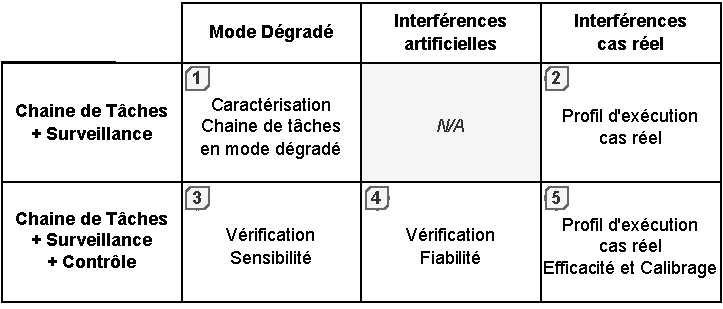
\includegraphics[width=0.8\linewidth]{tables/Table_Protocole_Implem}
		\end{table}
	
\pagebreak            
            
    \subsection{Spécification des paramètres de Contrôle}
    	L'étape \ctxt{1} de la calibration du mécanisme consiste à déterminer les grandeurs de paramétrage de ce dernier. Il est nécessaire de définir~: 
    	\begin{itemize}
    		\item $t_{sw}$ le temps de passage en mode dégradé ;
    		\item $T_{CCC}$ la période d'exécution du mécanisme de Surveillance et Contrôle ;
    		\item $rWCRT(\tau_{p})$ pour chaque tâche $\tau_p$ de la chaîne.
    	\end{itemize}
    
    	Le temps de passage en mode dégradé se calcule simplement de façon expérimentale, par mesures successives de déclenchement forcé du mode dégradé. Une valeur de borne maximale des mesures obtenue permet de garantir une estimation sûre de cette valeur. Dans les faits, cette valeur est relativement faible, voire négligeable. En effet, le passage en mode dégradé correspond à l'envoi d'un signal système qui met en pause les tâches non critiques. La durée de cette action dépend donc de deux éléments, d'abord du temps de réception du signal et ensuite du temps de mise en pause de la tâche. Ces derniers sont relativement faibles et la seule source de délai repose sur le temps de sauvegarde de contexte pour les tâches non critiques qui sont actuellement en cours d'exécution lors de la réception du signal.
    
    	\paragraph{\ctxt{1} -- Système exécuté en mode dégradé}
    	
    		Cette étape a pour objectif de déterminer deux des grandeurs susmentionnées. $T_{CCC}$ la période de vérification du mécanisme de contrôle. Et les différents $rWCRT(\tau_p)$ qui indiquent chacun la pire temps d'exécution restant garanti en mode dégradé pour la chaîne de tâche, selon le nombre de tâches restantes à exécuter pour la terminaison de la chaîne. 
    		
    		La chaîne de tâches est exécutée dans les mêmes conditions que le mode dégradé du système, avec le mécanisme qui est exécuté uniquement pour sa composante de Surveillance. Il convient donc de fixer en premier lieu le choix de $T_{CCC}$, qui est déterminé pour permettre au mécanisme implémenté de gérer la charge de réception des timestamps de terminaison des tâches critiques d'une part, et par le niveau de sensibilité à l'anticipation que l'on souhaite donner au mécanisme d'autre part. Il est ainsi hautement dépendant des spécifications de la partie critique du système. 
    		Pour donner une première valeur de période, nous nous focalisons sur la charge de réception. Il faut à chaque instant garantir qu'aucun timestamp ne soit perdu. Par conséquent, soit $L_{BUF}$ le nombre d'emplacements disponibles dans la mémoire tampon de réception des timestamps et $n$ le nombre de tâches critiques ayant pour périodes d'exécution $T_i, i \in [\![1,n]\!]$, alors la condition suffisante pour garantir le traitement de tous les timestamps est~:
    		\begin{equation}\label{eq:conditionsMemoireControle}
    			L_{BUF} \geq n  \quad \texttt{et} \quad T_{CCC} \leq \min{(T_i)}
    		\end{equation}
    		De cette façon, il est garanti qu'à chaque instant $t$, en pire cas le Core Control Component aura au maximum $n$ nouveaux timestamps à traiter, dans l'hypothèse --peu probable-- où toutes les tâches critiques se terminent en même temps. Une fois traités, ils sont ajoutés aux Traces d'Exécution actives gérée par la CCC pour le Contrôle.
    		De plus la récupération des timestamps doit être plus fréquente que l'occurrence de toute tâche critique, en particulier celle dont la période est la plus petite. En d'autres termes, le flux de traitement des timestamps par le mécanisme doit être supérieur au flux de terminaison des tâches critiques. 
    		Avec ces deux conditions, on a la garantie de ne perdre aucun timestamp envoyé. De fait, en considérant que chaque emplacement de la mémoire tampon correspond à une des tâches critiques, on a bien au moins 1 emplacement pour chaque tâche (première inéquation). Donc avec le mécanisme de contrôle qui s'exécute plus souvent que chacune des tâches critiques, on est sûr qu'il n'y aura pas plus d'un timestamp par tâche critique à gérer à chaque période de contrôle. On est donc sûr que la mémoire tampon n'aura pas de débordement et donc qu'aucun timestamp ne sera perdu. 
    		
    		Ces deux conditions de l'~\autoref{eq:conditionsMemoireControle} sont suffisantes, mais pas nécessaires. Cela fournit un premier couple de valeurs de période d'exécution et de taille de mémoire tampon simples et fonctionnels. Dans un cadre où la contrainte de mémoire disponible est très contraignante, il est probable que selon la chaîne de tâches étudiée, on puisse réduire taille de mémoire tampon, en calculant le nombre maximal de terminaison de tâches critiques possible durant une période de temps $T_{CCC}$.
    		Ou inversement, pour diminuer l'empreinte mémoire du mécanisme de surveillance et de contrôle, cette valeur de $T_{CCC}$ pourra être affinée en étape \ctxt{5}. Cela permet par la même occasion de jouer sur le niveau de sensibilité à l'anticipation du mécanisme, si nécessaire.
    		
    		Le mécanisme de surveillance est activé pour conserver les traces d'exécution de la chaîne de tâches $ET(j,t)$. 
    		Pour rappel, chaque trace d'exécution enregistre le timestamps de fin d'exécution de toutes les tâches de la chaîne selon le respect de la contrainte de précédence dans la chaîne. On reconstitue donc à partir de ces traces les temps d'exécution intermédiaires de la chaîne de tâche~: \\
    		pour chaque $p \in [\![1;n-1]\!], \quad ET(\,j\,,~t=succ^{\,p}(e_{1,j})~) = succ^{\,p}(e_{1,j}) - a_{1,j}$. \\
    		Comme on a pu le décrire en~\autoref{chap:3_PrincipeArchi}, les $e_{1,j}$ et $a_{1,j}$ correspondent respectivement aux dates de fin et d'activation du j\up{ème} job de la première tâche critique de la chaîne. Et $succ^{\,p}(e_{1,j})$ le timestamp de terminaison du p\up{ème} successeur du job d'entrée $\tau_{1,j}$ de la chaîne de tâches.
    		
    		En compilant tous les temps d'exécution intermédiaires obtenus, on peut en tirer des bornes maximales, qui correspondent alors aux différents $ rWCRT(\tau_p) $, on obtient~: \\
    		$\forall \ p \in [\![1\ ;\ n-1]\!], $, toutes les traces d'exécution obtenues :
    		
    		\begin{equation}
    			rWCRT(\tau_p) = \max_{j \in \mathbb{N^*}}\Big(~ET(\,j\,, succ^{\,p}(e_{1,j}) )~\Big) = \max_{j \in \mathbb{N^*}}\Big( succ^{\,p}(e_{1,j}) - a_{1,j} \Big) 
    		\end{equation} 
    	
    		Les $rWCRT(\tau_p)$ alimenteront donc la partie Contrôle du mécanisme pour son bon fonctionnement.
%           The task chain is then tested under a worst-case scenario. It is executed with the artificial system load, to stress as much as possible the task chain similarly to step \ctxt{2}. We get a baseline of the worst-case chain response time. This value is important because if the end-to-end deadline is always greater than the worst-case response time observed then the mechanism would be of no use (i.e. deadline never broken from temporal faults). This step gives a quantification of the task chain sensitivity to interferences and thus indicates the pertinence of using a Monitoring and Control Agent to manage them.
                    
                    
            \paragraph{\ctxt{2} -- Système complet avec Surveillance}
            
            Cette étape permet d'obtenir deux informations. La première essentielle est la valeur de $t_{SW}$, le temps de passage en mode dégradé. La seconde est la vérification de la pertinence d'utilisation du mécanisme de Surveillance et Contrôle. 
            
            De fait, en exécutant le système en condition normale de fonctionnement, adjoint au mécanisme de Surveillance sans activer le Core Control Component, il est possible de déclencher des transitions forcées aléatoires vers le mode dégradé, et d'en mesurer le temps de transition. Une borne supérieure aux valeurs mesurées permet de fixer $t_{SW}$.
            
            Par ailleurs, à l'image de ce qui a été fait dans le protocole de spécification d'un cas de test, en section~\ref{sec:pertinenceMecanisme}, on peut tirer profit de cette étape pour constater les potentielles fautes temporelles par dépassement de l'échéance bout-en-bout de la chaîne de tâches grâce à l'outillage de mesure permis par la Surveillance. Cette information de taux de dépassement d'échéance sur une mise en pratique expérimentale représentative offre une bonne base comparative pour les résultats ultérieurs qui seront obtenus après activation du mécanisme de contrôle.
            
            \smallbreak
            Suite à ces deux étapes, nous avons à disposition toutes les données et paramètres nécessaires à la mise en place du mécanisme complet de Surveillance et de Contrôle.
            L'objectif des étapes qui suivent dans le protocole est de quantifier l'efficacité du mécanisme. Cela est d'autant plus utile que les métriques proposées peuvent servir en retour pour ajuster les paramètres précédemment déterminés afin d'ajuster les propriétés et le comportement du mécanisme aux besoins du système. 
            
    \subsection{Calibration du Mécanisme de Contrôle}
    
    	\paragraph{\ctxt{3} -- Qualité du mécanisme}

    	Une première métrique d'analyse du mécanisme est la \textbf{qualité}. Cela consiste à identifier dans quelle mesure le mécanisme serait trop sensible, et donc déclencherait des passages en mode dégradé non nécessaires.
    	
    	Cette mesure est relativement complexe à obtenir de façon parfaite, dans le sens où cela nécessiterait d'identifier précisément pour chaque décision du mécanisme, si le passage en mode dégradé était nécessaire ou non. Hors, il n'est pas possible d'avoir un oracle parfait qui donnerait le résultat en cas de conservation du mode nominal à chaque instant où la décision a été prise. 
    	
    	Par conséquent, la mesure que nous allons considérer ici consiste à identifier les passages en mode dégradé dans un cas où l'on sait qu'il ne devrait en avoir aucun, c'est-à-dire en isolation. 
    	Un test que nous réalisons consiste donc à exécuter le système directement en mode dégradé, avec les tâches non critiques qui ne sont pas exécutées, mais le mécanisme complètement actif.
    	De cette façon, on mesure la qualité du mécanisme à partir de son comportement dans un cadre où \textit{a priori} il ne devrait pas déclencher de mode dégradé, par absence d'interférences. Tout passage en mode dégradé dans ces conditions sera alors \textit{de facto} un faux positif.
    	En dénombrant les passages en mode dégradé dans de telles conditions expérimentales, on a alors une première idée de la qualité du mécanisme. Plus le nombre de faux positifs sera élevé, moins la qualité sera bonne.
    	
    	Aussi, il existe des variables d'ajustements pour influer sur la qualité du mécanisme. Le principal facteur est sa période d'exécution $T_{ccc}$. De fait, plus le nombre de changements de modes est élevé, plus cela signifie que le mécanisme est sensible. Cela peut être alors dû à deux éléments : 
    	\begin{itemize}
    		\item Soit la période d'exécution du mécanisme de contrôle est trop grande, ce qui fait que la constante $W_{MAX}$ dans~\autoref{eq:safe_cond} de l'anticipation est trop prépondérante. Cela provoque une anticipation qui se base sur un point de contrôle suivant trop lointain. La vérification de l'absence de risque de dépassement prend en considération une période avant le prochain point de contrôle trop grande, ce qui augmente d'autant la potentialité d'un risque de dépassement. Pour obtenir une bonne anticipation du risque de viol de l'échéance la prise de décision devrait se baser en premier lieu sur les grandeurs dynamiques du système, qui évoluent au fil de l'exécution, donc $RT(t)$ et $rWCRT(t)$. En d'autres termes, plus la période de contrôle est grande, plus le risque de dépassement anticipé entre deux périodes est grand, et donc plus le mécanisme est sensible. Diminuer la période améliore la sensibilité, au coût d'une plus grande utilisation du CPU.
    		\item Soit les ordres de grandeur impliqués entre les temps d'exécution des tâches avec et sans perturbations sont trop proches au regard des autres grandeurs du système (période de surveillance notamment), ce qui rend la différenciation entre un cas à risque et un cas nominal bien trop subtil pour être discriminé par le mécanisme. Cela peut être dû aux estimations trop pessimistes qui ont été faites sur les pires temps de réponse restants, autrement, il est possible que l'échéance fixée soit simplement trop stricte et en conséquence trop proche des temps de réponse constatés lors d'un fonctionnement sans aucune interférence. Auquel cas ce genre de mécanisme n'est pas adapté et il faudra se contenter des méthodes plus classiques de contrôle statique au détriment de l'optimisation de la puissance de calcul.
    	\end{itemize}
    	Dans l'idéal, il faudrait qu'aucun déclenchement de mode dégradé ne soit constaté dans ce cadre-ci. Dans de telles conditions, cela indique potentiellement qu'une plus grande période d'exécution du mécanisme est possible, afin d'alléger son empreinte sur l'utilisation du processeur. Cela reste bien entendu conditionné à la capacité de réception de tous les timestamps bien entendu, selon la condition présentée en ~\autoref{eq:conditionsMemoireControle}.
    	
    	\paragraph{\ctxt{4} -- Fiabilité du Mécanisme}
        En exécutant la chaîne de tâches critique avec le Contrôle opérationnel dans un contexte où le processeur est le plus stressé possible en terme d'interférence, il est possible de mesurer la \textbf{fiabilité} du mécanisme.
        Dans un tel contexte pire cas, il est possible de vérifier si les paramètres de contrôle choisis sont corrects. Si tel est le cas, on ne devrait observer aucun dépassement d'échéance bout-en-bout lors de ces tests. 
        S'il advenait que l'échéance de temps de réponse bout-en-bout ne soit pas respectée un certain nombre de fois, alors il serait essentiel d'approfondir la question pour remonter aux raisons de ces fautes.
        
		Il peut y avoir deux explications à de tels dépassements. Il peut s'agir simplement d'une sous estimation des $rWCRT(\tau_p) $, qui a mené à un déclenchement du mode dégradé trop tardif.
        Cela doit pouvoir s'observer via la trace d'exécution de la chaîne de tâches qui a conduit au dépassement. On devrait observer un profil d'exécution dans les tranches hautes de temps de réponse habituellement observés pour la chaîne de tâches (et donc proche, mais inférieur aux valeurs de $rWCRT(\tau_p)$ paramétrées), mais pas suffisamment pour que le déclenchement du mode dégradé se soit fait assez tôt.
        
        En revanche si cela n'est pas constaté et qu'il y a dépassement d'échéance malgré le mécanisme de Contrôle semble qui s'être déclenché dans les temps, alors il est possible que ce soit dû à des facteurs non contrôlés par le mécanisme. Plus spécifiquement, il peut s'agir de retards d'exécution qui ne proviennent pas des interférences matérielles liées aux tâches non-critiques.
        Si ce cas est souligné ici, c'est parce qu'il est vraisemblable lorsque ce genre de mécanisme est utilisé dans un environnement complexe où tout ce qui se produit au niveau du système d'exploitation n'est pas parfaitement maîtrisé. Cela est particulièrement le cas avec l'usage de plus en plus fréquent de distributions Linux pour les systèmes embarqués. Plusieurs travaux tels que~\cite{allende_towards_2019} ou encore \cite{sivakumar_automotive_2020} et \cite{serra_architecture_2020} se sont intéressés aux conditions de mise en place d'un tel système pour du temps-réel, les difficultés que cela implique ainsi que ce que l'on peut attendre de Linux dans ces conditions. Cette étape de vérification de la fiabilité peut donc permettre de soulever des problèmes externes propres au matériel ou au logiciel sous-jacent, qui devront être résolus par ailleurs. Cela peut provenir de l'utilisation de drivers inadaptés, ou de l'exécution de code non stoppé avec les tâches non critiques (tâches système, typiquement). Dans un contexte industriel avec un OS dédié, cette seconde source ne devrait logiquement pas exister. 
                    
		\paragraph{\ctxt{5} -- Système complet avec mécanisme de contrôle}
		 Pour finir, la dernière étape du protocole de calibration et d'implémentation du mécanisme consiste simplement à exécuter la totalité du système en mode nominal, accompagné du mécanisme de surveillance et de contrôle. 
		 Cette dernière phase d'essai a, elle aussi, pour objectif d'apporter des métriques d'analyse de fonctionnement du mécanisme. Nous avons mesuré jusqu'à présent la fiabilité et la qualité de ce dernier. Il reste alors la \textbf{performance}, qui regarde dans quelle mesure nous réussissons à conserver l'exécution des tâches non critiques malgré l'ajout du mécanisme de contrôle.
		 En réalisant ce test dans les mêmes conditions que l'étape \ctxt{2} où la partie Contrôle était inactive, on peut donc comparer le temps d'exécution et le nombre de jobs réalisés pour chaque tâche non critique, au regard de la diminution du nombre de dépassements d'échéances. On devrait normalement constater un taux de dépassement de l'échéance qui devient nul en cas d'une fiabilité de 100\%.
		 Par la même occasion, on peut mesurer le temps d'exécution moyen du mécanisme de surveillance et contrôle en fonctionnement nominal, de façon à vérifier que son empreinte d'utilisation du CPU est non significative et n'empiète donc pas sur les performances globales, ce qui serait bien entendu contre-productif.
		 
		 Cette étape est enfin l'occasion de faire varier les paramètres de configuration du Contrôle en réitérant sur les 2 étapes précédentes, pour ajuster les performances mesurées du mécanisme aux besoins spécifiques de l'application si nécessaire. Ainsi il sera possible de modifier la période d'exécution du Contrôle soit  pour diminuer son utilisation du CPU dans le cas d'un taux d'utilisation considéré trop élevé, soit parce que l'on a constaté une sensibilité trop élevée, par un nombre de faux positifs trop grand.
		 Il est aussi possible d'accepter de façon exceptionnelle des dépassements de l'échéance bout-en-bout, dans un modèle où la chaîne serait à temps-réel souple typiquement ou si l'on veut garantir un niveau de Qualité de Service (\textit{QoS}) comme cela a pu être développé dans des études comme~\cite{lin_maximizing_2006}. Pour ce faire, on peut revoir les valeurs de $rWCRT(\tau_p)$ à la baisse. Cela revient à fixer les pires temps d'exécution restant garantis en mode dégradé à des valeurs plus optimistes. Par conséquent, la sensibilité du mécanisme sera allégée au détriment de dépassements d'échéance de façon occasionnelle malgré le passage en mode dégradé, typiquement quand le temps de réponse en mode dégradé sera situé juste au dessus des nouveaux seuils de $rWCRT(\tau_p)$ qui ont été abaissés. Cela donnera alors une fiabilité inférieure à 100\% de garantie de l'échéance, mais qui peut être ajustée expérimentalement pour rester à un taux d'occurrences maîtrisé. Il serait alors possible par calcul probabiliste de fixer une baisse de ces valeurs pour obtenir au niveau souhaité de taux de défaillance temporelle sur la chaîne de tâches critiques, typiquement.
		 
		 Ces ajustements des paramètres du mécanisme sont des possibilités offertes par ce dernier, hautement dépendantes de besoins spécifiques. Nous étudierons plus en détail l'influence de variation de ces valeurs dans la suite des travaux. Le protocole expérimental d'analyse du mécanisme étant clos ici.    	
                	
                	
\section{Protocole expérimental global}
    
    Pour la suite de nos travaux, comme l'on peut s'en douter nous avons dû mettre en œuvre les deux protocoles expérimentaux présentés ici. En premier lieu le protocole de spécification d'un cas de test mis en application sur une suite logicielle de benchmarking. Et ensuite le protocole d'implémentation du mécanisme de surveillance et de contrôle sur le cas de test précédemment spécifié. Par conséquent, nous présentons en conclusion de cette partie le tableau récapitulatif expérimental, dans le cas où ces 2 méthodes doivent être employées successivement.
    
    Il est à noter que les deux protocoles se recoupent en partie, dans les conditions expérimentales de test de la chaîne de tâches critiques. Il s'agit de la seconde ligne du~\autoref{tab:tableprotocoledesign} où la chaîne de tâches est caractérisée, qui propose les mêmes conditions expérimentales que la première ligne du~\autoref{tab:tableprotocoleImplementation}. La nuance à noter est que là où le protocole de Spécification propose une caractérisation de la chaîne de tâches \textit{en isolation}, dans le cadre de l'implémentation du mécanisme de contrôle, ces conditions de test doivent correspondre au cas exact dans lequel sera le système en mode dégradé. Il s'agit alors d'un cas où la chaîne de tâche est isolée d'interférences des tâches non critiques, mais cela implique aussi une configuration spécifique des tâches critiques, notamment sur leur allocation physique sur les cœurs du processeur. 
    En bref, tout cela pour exprimer que la caractérisation de la chaîne de tâche doit se faire dans les mêmes conditions que celles qui seront impliquées lors d'un passage en mode dégradé par le mécanisme de contrôle.
    
    \begin{table}[ht]
    	\centering
    	\caption{Protocole "Complet" de Spécification, Caractérisation et Analyse}
    	\label{tab:tableprotocoleComplet}
    	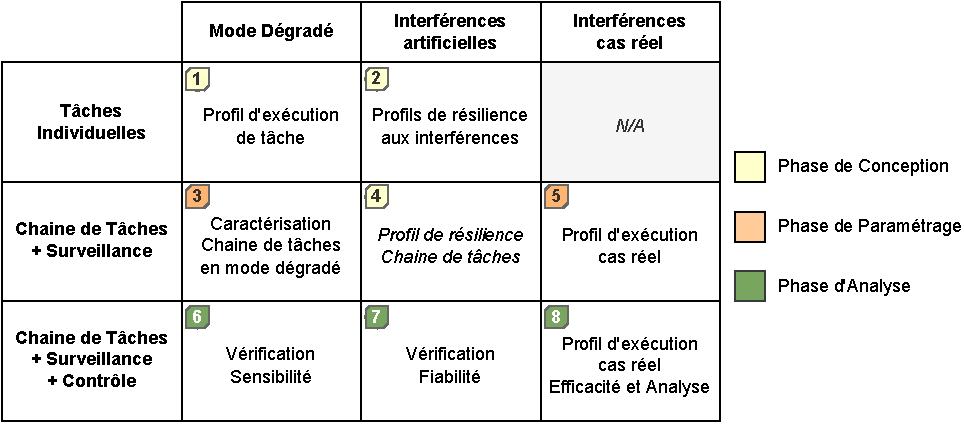
\includegraphics[width=\linewidth]{Table_Protocole_Complet}
    \end{table}

   	En bilan, nous avons donc le~\autoref{tab:tableprotocoleComplet} qui donne 3 Phases expérimentales : la Conception, le Paramétrage et l'Analyse. 
   	
   	Lors de la phase de Conception, sont testées successivement les tâches de façon individuelle pour en obtenir une caractérisation temporelle. Cela permet d'avoir une meilleure connaissance des temps d'exécutions des tâches et de leur propension à introduire et/ou recevoir des interférences sur l'utilisation de ressources partagées. Dans le cas où il ne s'agit pas d'un jeu de tâches déjà spécifié pour un système industriel, il s'agit aussi de constituer la sélection d'un jeu de tâches de test à partir de tâches provenant d'un benchmark ou autre. Cela permet de spécifier les tâches non critiques et les tâches critiques sous forme d'une chaîne de tâches. Dans cette éventualité, la phase de conception propose enfin la vérification des choix effectués notamment en termes de taux d'utilisation du processeur et de la présence manifeste d'interférences qui peuvent mener à des dépassements d'échéances.
   	
   	Vient ensuite la phase de Paramétrage, qui repose sur l'exécution de la chaîne de tâches critiques uniquement pour déterminer les paramètres du mécanisme de Surveillance et Contrôle.
   	
   	Pour finir, la phase d'Analyse intègre la chaîne de tâches avec l'ajout du mécanisme complet. Chaque test est soumis soit à aucune interférence matérielle spécifique (cas en mode dégradé), soit avec des interférences imposées de façon artificielle pour s'approcher d'un "pire cas" de charge, soit avec la charge réelle qui inclut les interférences inhérentes à toutes les tâches du système, notamment les tâches non critiques. De ces tests, on est en mesure de définir les propriétés du mécanisme de Surveillance et Contrôle selon des critères de Fiabilité, Qualité et Performance tel que présentés précédemment. 
   	

   	
\ifdefined\included
\else
\bibliographystyle{StyleThese}
\bibliography{these}
\end{document}
\fi
